
	% !TEX options=--shell-escape
	\documentclass{article}
	\usepackage{amsmath,amssymb}
	\usepackage[inline]{enumitem}
	\usepackage{blindtext}
	\usepackage{booktabs}
	\usepackage{graphicx}
	\usepackage{xcolor}
	\usepackage[vmargin = 1.5in, top = 1in, bottom = 1.2in, letterpaper]{geometry}
	\usepackage{listings}
	\usepackage{courier}
	\usepackage{multicol}
	\usepackage{multirow}
	\usepackage{bm}
	\usepackage{subcaption}
	\usepackage{minted}
	\usepackage{fvextra}
	\definecolor{bg}{rgb}{0.95,0.95,0.95}
	\newminted{r}{mathescape, breaklines, linenos = true, bgcolor = bg, breaksymbolleft=\carriagereturn}
	\usemintedstyle{tango}
	% \lstset{
	% basicstyle = \small\tt,
	% keywordstyle = \tt\color{blue},
	% commentstyle = \it\color[cmyk]{1,0,1,0},
	% stringstyle = \tt\color[RGB]{128,0,0},
	% %frame = single,
	% backgroundcolor = \color[RGB]{245,245,244},
	% breaklines,
	% extendedchars = false,
	% xleftmargin = 2em,
	% xrightmargin = 2em,
	% aboveskip = 1em,
	% tabsize = 4,
	% showspaces = false
	% }
	\newcommand\inner[2]{\left\langle{#1},{#2}\right\rangle}
	\DeclareMathOperator{\Corr}{Corr}
	\DeclareMathOperator{\Cov}{Cov}
	\DeclareMathOperator{\Var}{Var}
	\DeclareMathOperator{\E}{E}



	\begin{document}
	
	% \newfontfamily\courier{Courier New}

	
	\title{STAT 501 Homework 1}
	\author{Gaussian}
	\maketitle
	
	\begin{enumerate}[leftmargin = 0 em, label = \arabic*., font = \bfseries]
	\item 
	\begin{enumerate}
		\item 
		Read the dataset
		\begin{rcode}
senators<-read_xls("senate_voting_data.xls")		
		\end{rcode}

		\item 
		Plot Andrews' curves
		\begin{rcode}
senators.names<-names(senators)[-c(1,2)]
rev.party.state.names<-lapply(X=strsplit(gsub(patterns = "[.]", replacement = "",x=senators.names), strsplit = " "),FUN = rev)

senators.party <- lapply(X = rev.party.state.names, FUN = function(x)(unlist(x)[1]))
senators.party <- unlist(senators.party)

senators.last.names <- lapply(X = rev.party.state.names, FUN = function(x)(unlist(x)[4]))
senators.last.names <- unlist(senators.last.names)


#Create new data.frame for plotting
senators_new <- as.data.frame(t(senators[,-c(1,2)]))

colnames(senators_new) <- NULL
rownames(senators_new) <- NULL

senators_new <- data.frame(senators_new, party = senators.party)

# Use the codes from Canvas
source("ggandrews.R")

# Display the Andrews' curves
ggandrews(senators_new, type = 2, clr = 543, linecol = c("blue", "purple", "red"))		
		\end{rcode}

		Andrew's Curves for senators is shown in Figure~\ref{1b}.
		\begin{figure}[!htb]
		\centering
			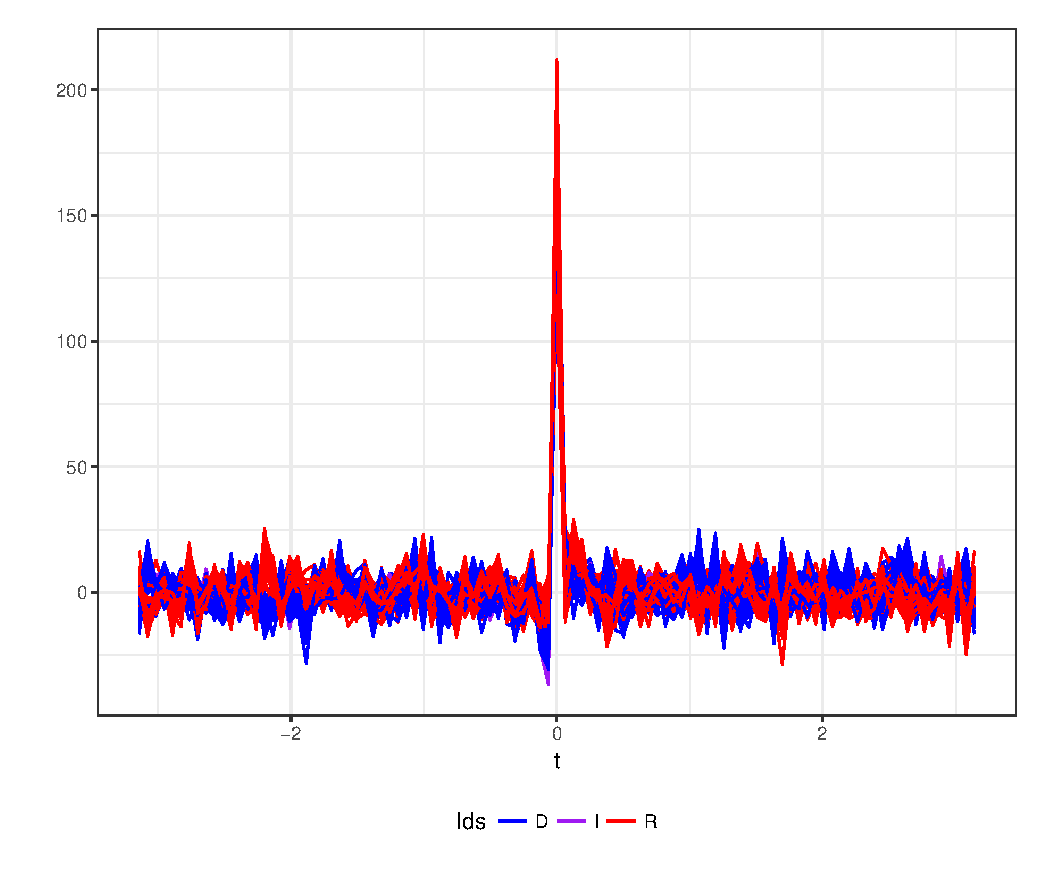
\includegraphics[width = 0.7\textwidth]{1b.eps}
			\caption{Andrew's Curves for senators}
			\label{1b}
		\end{figure}
		From Andrews' curves we can see that for each party the curve follows a similar pattern, so senators within each party have similar voting preferences. We can also see curves from three different parties are mixed together, so it would be hard to distinguish the senator's party from the voting preference. 
		
	\end{enumerate}
	
	\newpage
	\item 
	\begin{enumerate}
		\item 
		Radial visualization and star coordinates
		\begin{rcode}
library(lattice)
require(dprep)
sclerosis <- read.table("sclerosis.dat", header=F)

p <- dim(sclerosis)[2]
sclerosis[, p] <- as.factor(ifelse(sclerosis[,p] == 0, "normal", "sclerosis"))

colnames(sclerosis) <- c("Age", "TS1", "DS1", "TS2", "DS2", "Disease")

# Use codes from Canvas
source("radviz2d.R")

# Display the radial visualization plot 
radviz2d(dataset = sclerosis, name = "Sclerosis")

# Use the codes from Canvas 
source("starcoord.R")

#Display the star coordinates
starcoord(data = sclerosis, class = TRUE)
		\end{rcode}
        
        Plot for radial visualization is shown in Figure~\ref{2arad} and plot for star coordinates is shown in Figure~\ref{2acoord}. From the radial visualization, we can see there is more variability in age within the ``normal'' group than that of ``sclerosis'' group. And the total response for stimuli S1 and S2 are similar in both groups. The differences of response for S1 and S2 are also similar in both groups. From the star coordinates plot, we can also see that the ``normal'' group varies more that the ``sclerosis'' group in age. We can also see ``normal'' group varies less than the ``sclerosis'' in other dimensions and values for those dimensions are smaller.  
		\begin{figure}[!htb]
			\centering
			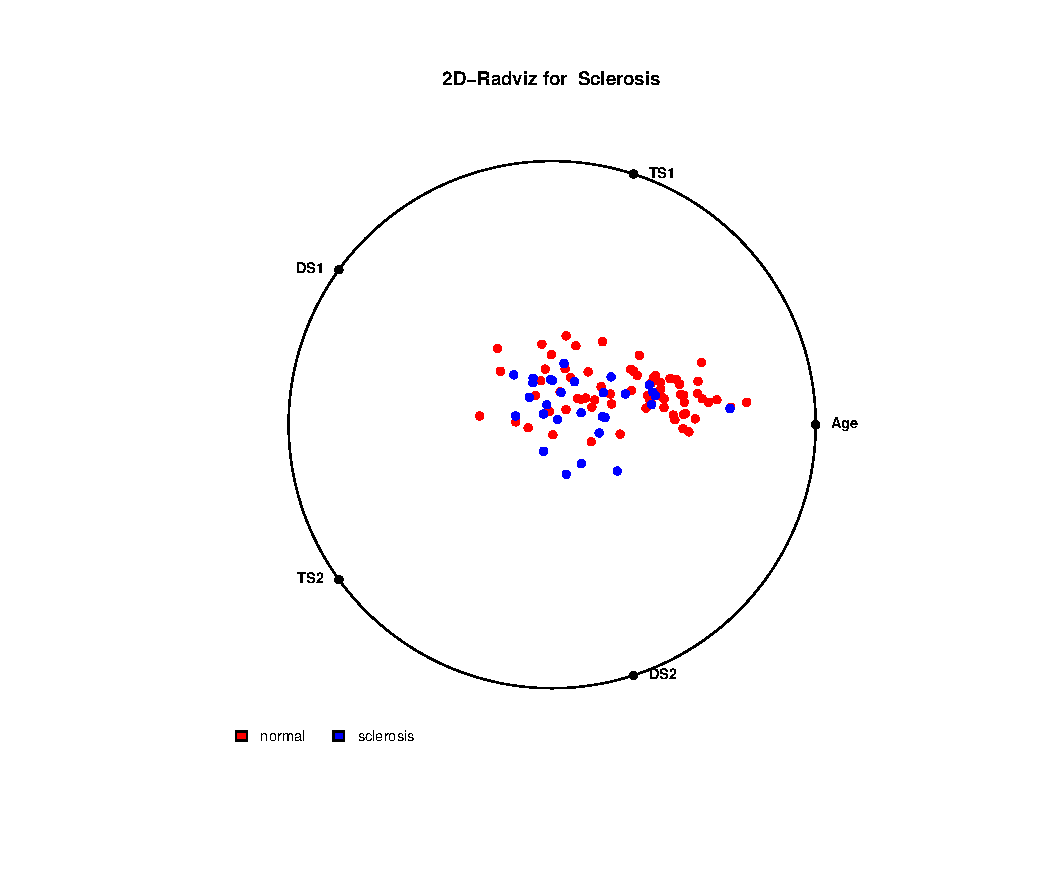
\includegraphics[width = 0.7\textwidth]{2a.eps}
			\caption{Radial visualization for sclerosis data}
			\label{2arad}
		\end{figure}
		\begin{figure}[!htb]
			\centering
			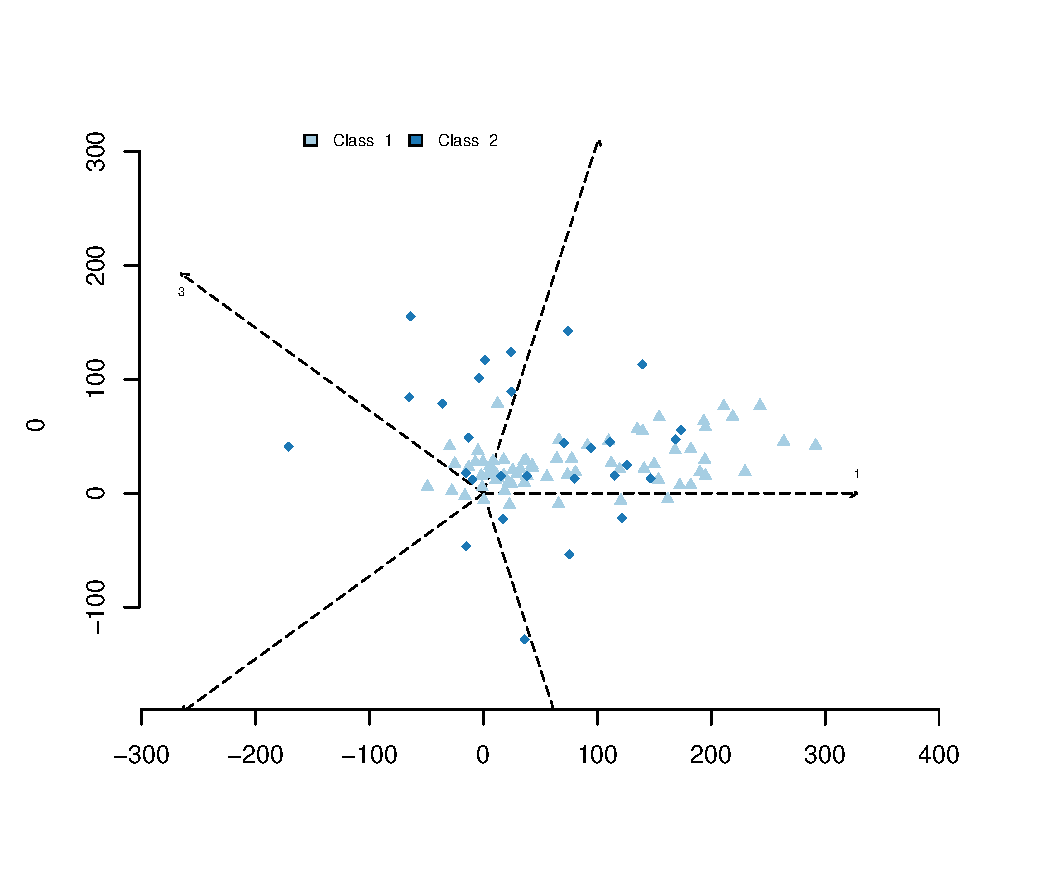
\includegraphics[width = 0.7\textwidth]{2astarcoord.eps}
			\caption{Star coordinates for sclerosis data}
			\label{2acoord}
		\end{figure}
		
\newpage
		\item 
		Calculate the means for each group
		\begin{rcode}
normal_mean<-colMeans(sclerosis[sclerosis[,p]=="normal", -p])
normal_mean

sclerosis_mean<-colMeans(sclerosis[sclerosis[,p]=="sclerosis",-p])
sclerosis_mean
		 \end{rcode} 
		 Means for group ``normal'':
		 \begin{verbatim}
       Age        TS1        DS1        TS2        DS2 
 37.985507 147.289855   1.562319 195.602899   1.620290 		 
		 \end{verbatim}
		 Means for group ``sclerosis'':
		 \begin{verbatim}
      Age       TS1       DS1       TS2       DS2 
 42.06897 178.26897  12.27586 236.93103  13.08276 
		 \end{verbatim}

		 \item 
		 Display the Chernoff faces 
		 \begin{rcode}
sclerosis_mean_data <- as.matrix(rbind(normal_mean, sclerosis_mean))
library(TeachingDemos)
faces(sclerosis_mean_data, labels = c("normal", "sclerosis"))
		 \end{rcode}
		 The Chernoff faces for the two groups are shown in Figure~\ref{2c}.
		 \begin{figure}[!htb]
		 	\centering
		 	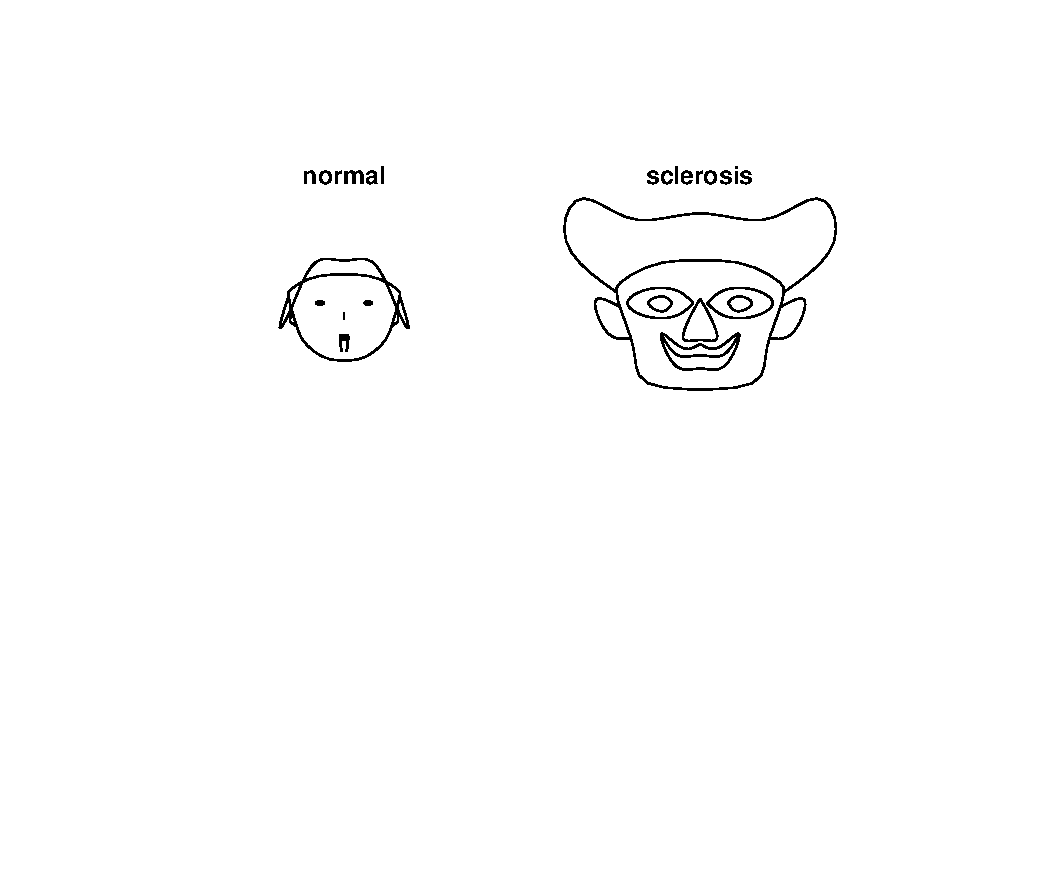
\includegraphics[width=0.7\textwidth]{2c.eps}
		 	\caption{Chernoff faces for two groups of sclerosis data}
		 	\label{2c}
		 \end{figure}
\newpage
		 \item 
		 Display the correlation matrix for each group. 
		 \begin{rcode}
source("plotcorr.R")
# normal
plot.corr(xx = sclerosis[sclerosis[,p]=="normal", -p])

# sclerosis
plot.corr(xx = sclerosis[sclerosis[,p]=="sclerosis", -p])
		 \end{rcode}
		 Correlation plots are shown in Figure~\ref{2d}.
		 \begin{figure}[!htb]
		     \centering
		 	\begin{subfigure}[b]{0.5\textwidth}
		 	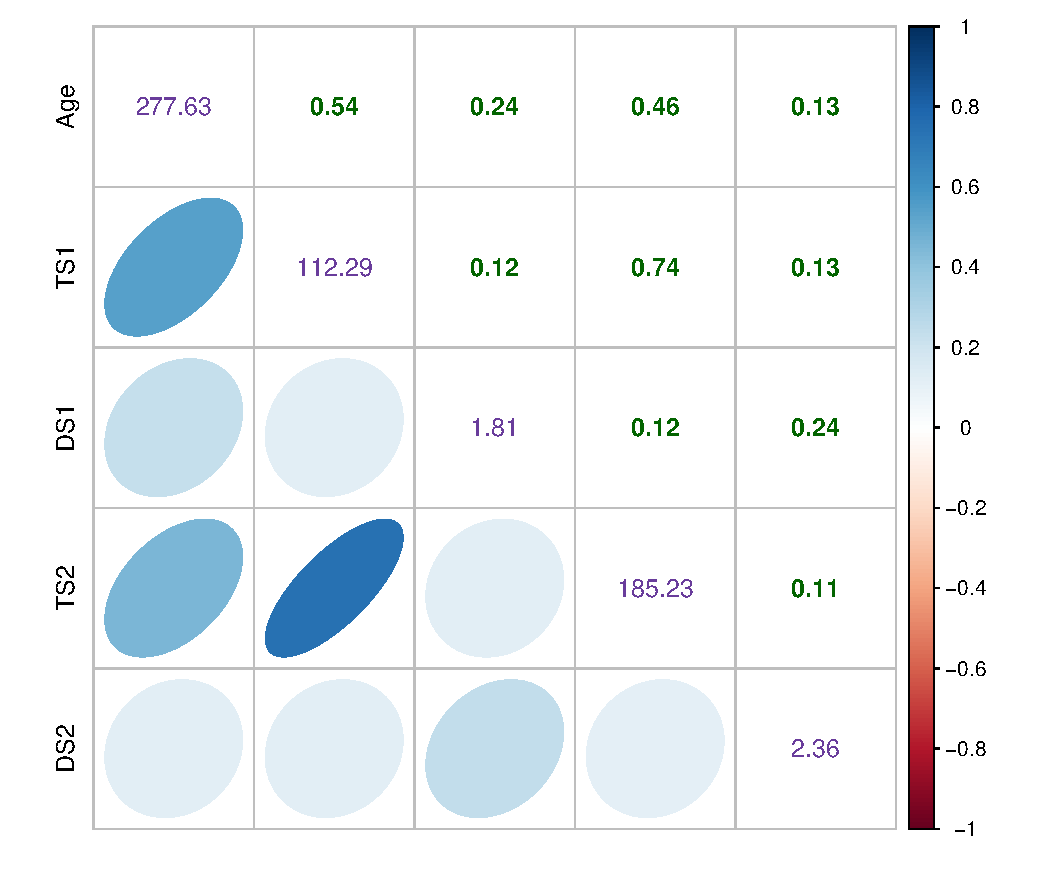
\includegraphics[width = \textwidth]{2dnormal.eps}
		 	\caption{normal}
		 	\end{subfigure}%
		 	\begin{subfigure}[b]{0.5\textwidth}
		 	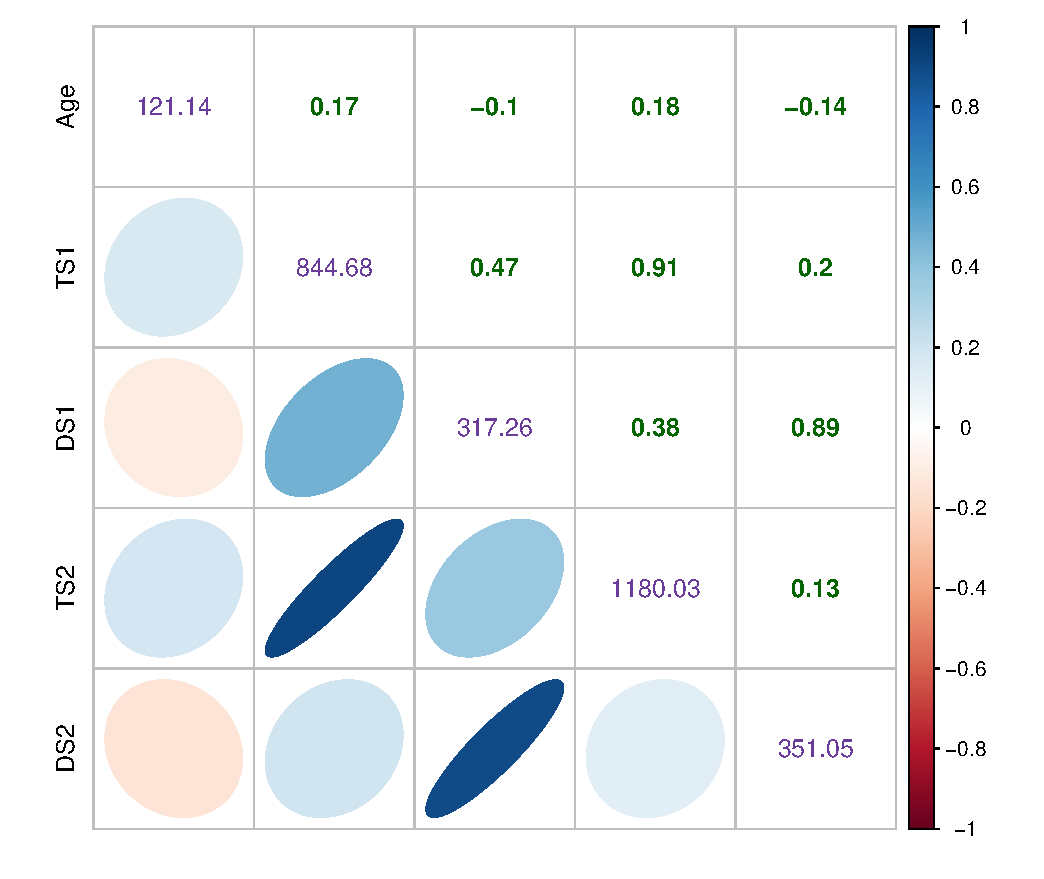
\includegraphics[width = \textwidth]{2dsclerosis.eps}
		 	\caption{sclerosis}
		 	\end{subfigure}
		 	\caption{Correlation plots for two groups}
		 	\label{2d}
		 \end{figure}
        We can see for both groups, total response with stimuli S1 and total response with stimuli S2 are highly correlated. For the ``sclerosis'' group we can also see difference in response with stimuli S1 and stimuli S2 are also highly correlated. Total response and age for ``normal'' group shows a stronger association than ``sclerosis'' group. We can also see the variance of age for ``normal'' group is larger than that of ``sclerosis'' group, and the variances for ``normal'' group are smaller than those of ``sclerosis'' group in other dimensions. 
	\end{enumerate}
	
	\item 
	\begin{enumerate}
		\item 
		Formulate the correlation plot
		\begin{rcode}
#Read the dataset
Tornado<-read.table(file ="https://www.nssl.noaa.gov//users/brooks//public_html//
feda//datasets//tornf1p.txt", col.names = c("year", "jan", "feb", "mar","apr", "may","jun","jul", "aug","sep", "oct", "nov", "dec"))
#Create correlation plot
source("plotcorr.R")
plot.corr(Tornado[2:13])
		\end{rcode}

		The correlation plot is shown in Figure~\ref{3a}. Generally it is observed that months next to each other or near to each other like Jan-Feb, Jan-March has positibe correlation while month far away from each other/ in oppite season o year like Jan-June, Jan-July has negative correlation although it is not true for all the cases. From the correlation plot it is also observed that the variance is high for months during spring/early summer Apr-June compared to other months.
		\begin{figure}[!htb]
			\centering
			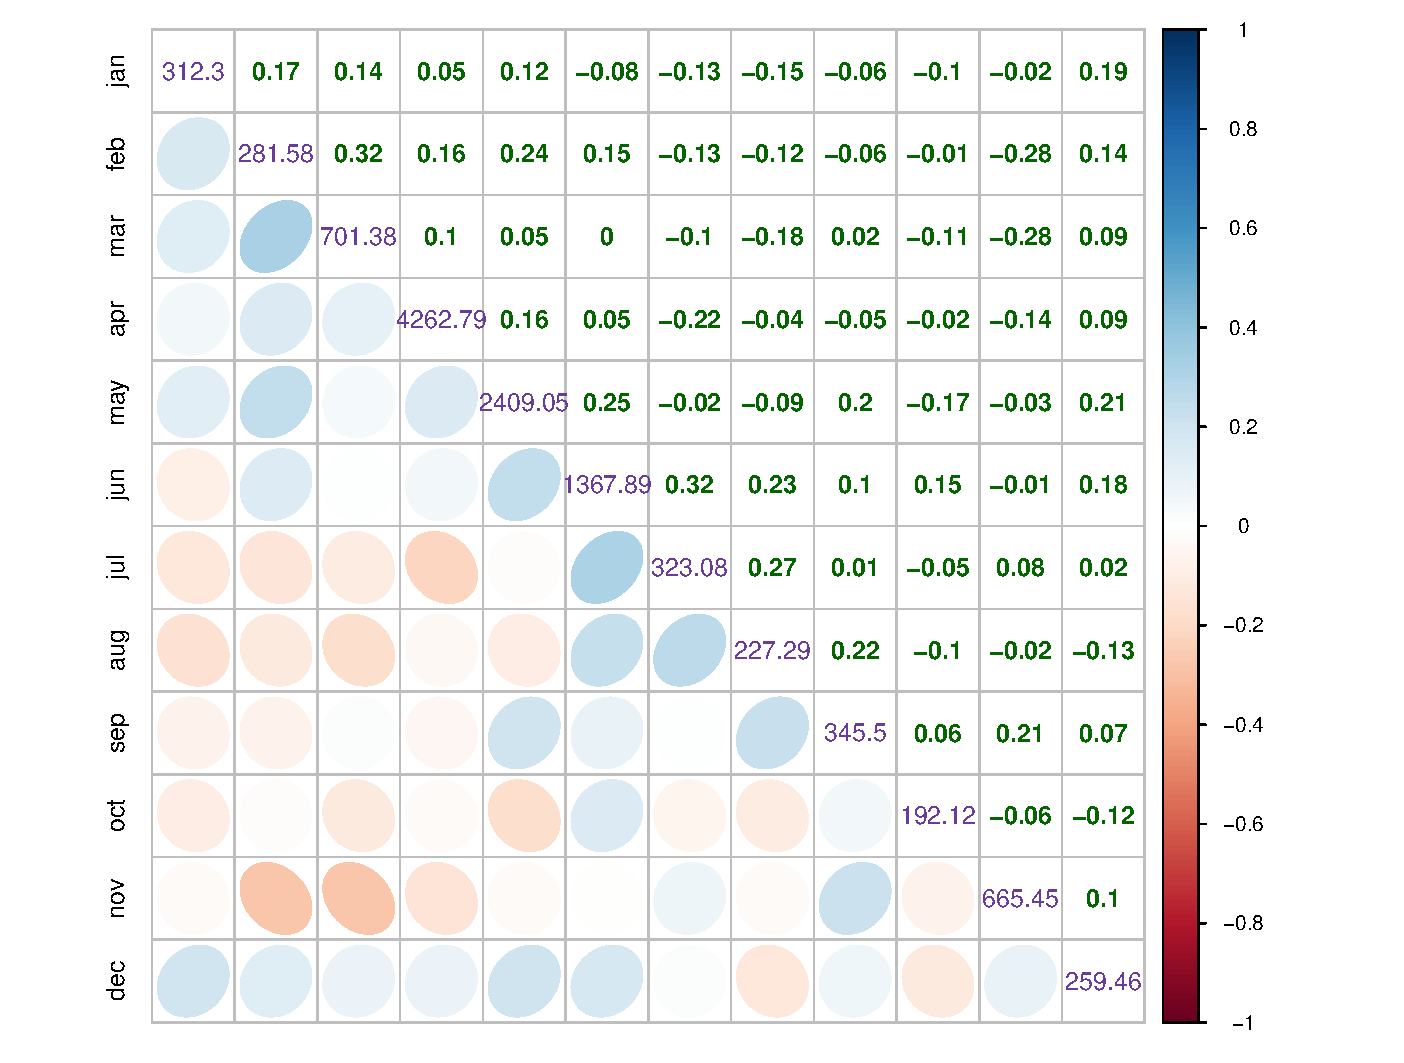
\includegraphics[width = 0.7\textwidth]{3a.eps}
			\caption{Correlation plot for Tornado data}
			\label{3a}
		\end{figure}

\newpage
		\item 
		\begin{enumerate}
			\item 
			Parallel-coordinates plot for each group
			\begin{rcode}
#Create 3 group and a column of group in the dataframe
Tornado$Period<-cut(x = Tornado$year,breaks=c(1954,1974,1994,2014),labels = c("I","II","III"),include.lowest = F)

#Create parallel plot with colour by the group
source("parcoordplot.R")
parcoordplot(xx =Tornado[-1,2:13],cl = as.factor(Tornado$Period[-1]),FUN=mean,alpha = 0.2)
			\end{rcode}
			The parallel-coordinates plot is shown in Figure~\ref{3bi}.
		\begin{figure}[!htb]
			\centering
			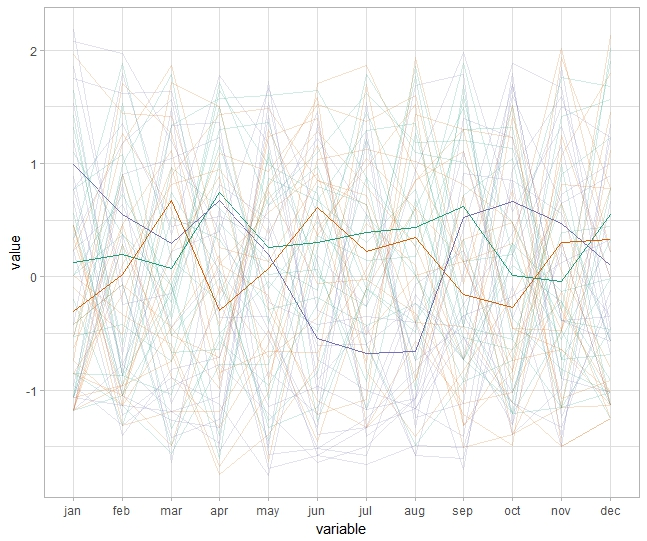
\includegraphics[width = 0.7\textwidth]{3bi.jpeg}
			\caption{Parallel-coordinates plot for Tornado data}
			\label{3bi}
		\end{figure}
		From the parallel plot along with superimposed mean it can be seen that during different period the frequency of tornado varied largely across the months. For example during third period the frequency was very low from June to August while it was high during 1st and 2nd period. Any specific pattern however is hard to observe due to the variation.

\newpage
		\item 
		Create survey plots ordered by each of 12 months
		\begin{rcode}
source("surveyplot.R")
for (i in 1:12){
  surveyplot(cbind(Tornado[,2:13], as.numeric(as.factor(Tornado[,14]))), order = i)}	
		\end{rcode}
        
        \begin{figure}[!htb]
            \centering
        	\begin{subfigure}[b]{0.3\textwidth}
        	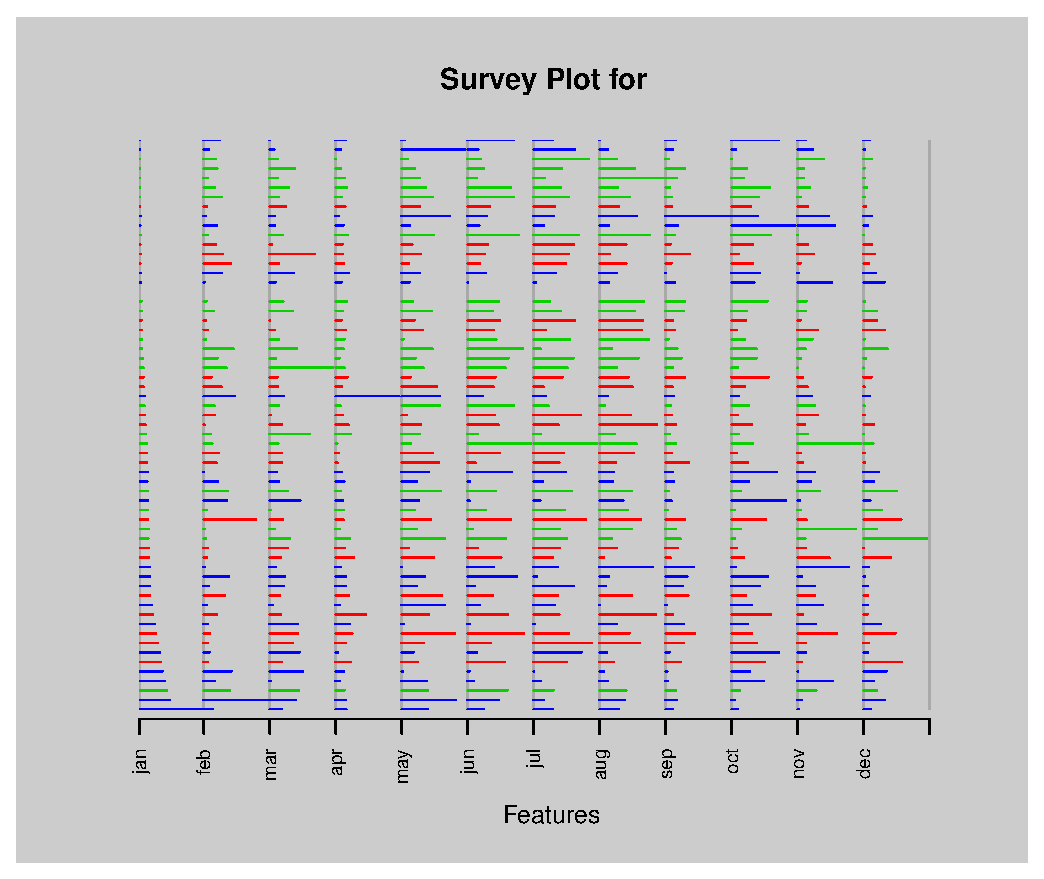
\includegraphics[width = \textwidth]{3cii1.eps}
        	\caption{Jan}
        	\end{subfigure}%
        	\begin{subfigure}[b]{0.3\textwidth}
        	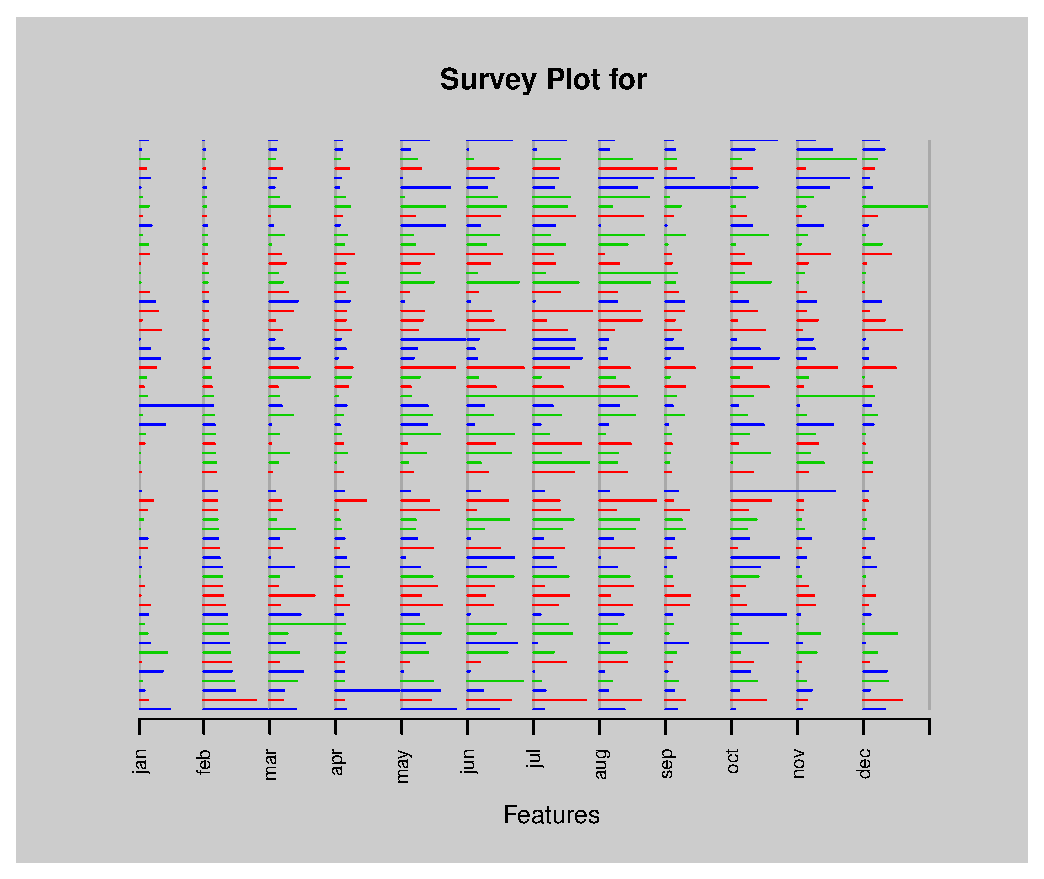
\includegraphics[width = \textwidth]{3cii2.eps}
        	\caption{Feb}
        	\end{subfigure}%
            \centering
        	\begin{subfigure}[b]{0.3\textwidth}
        	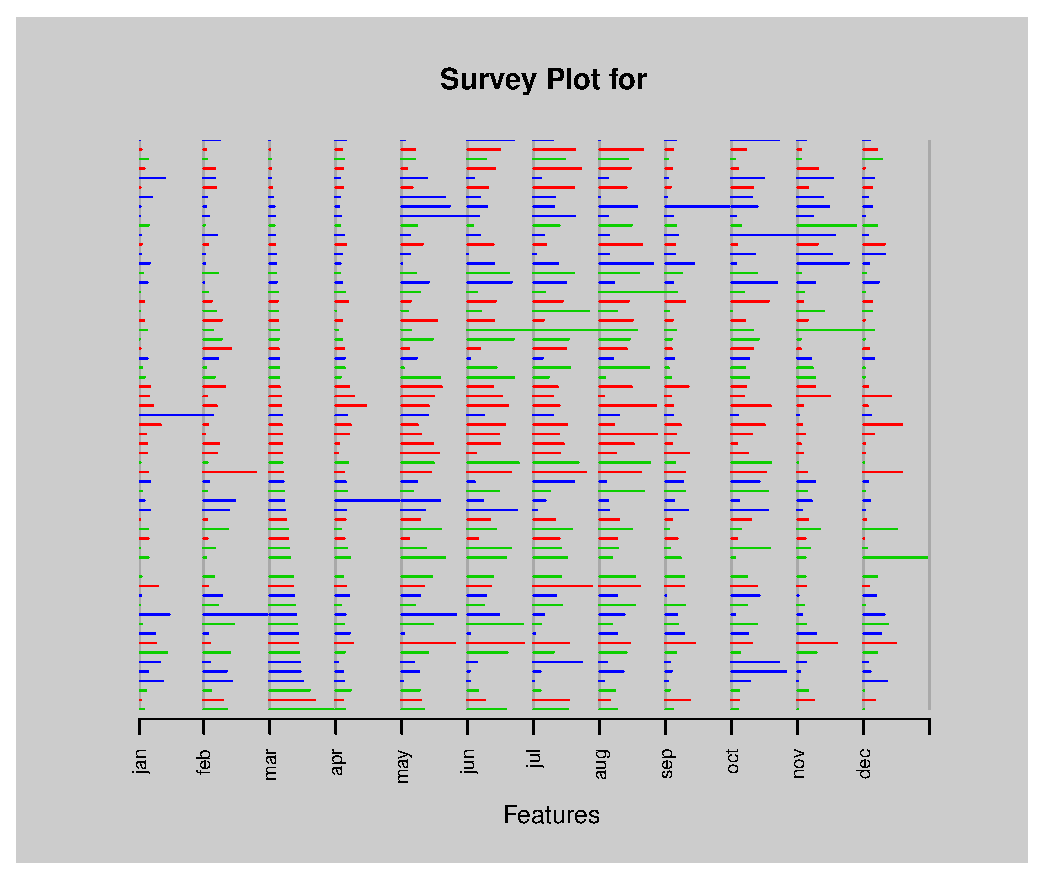
\includegraphics[width = \textwidth]{3cii3.eps}
        	\caption{Mar}
        	\end{subfigure}\\
        	\begin{subfigure}[b]{0.3\textwidth}
        	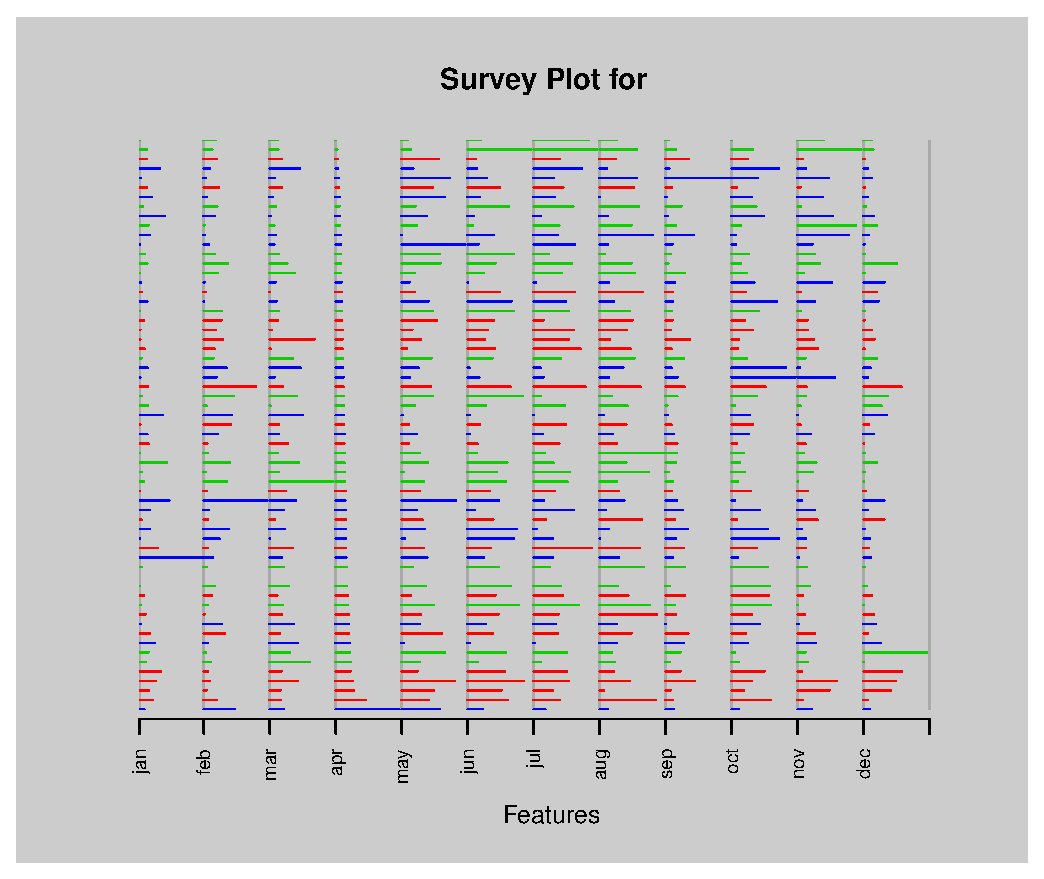
\includegraphics[width = \textwidth]{3cii4.eps}
        	\caption{Apr}
        	\end{subfigure}%          
        	\begin{subfigure}[b]{0.3\textwidth}
        	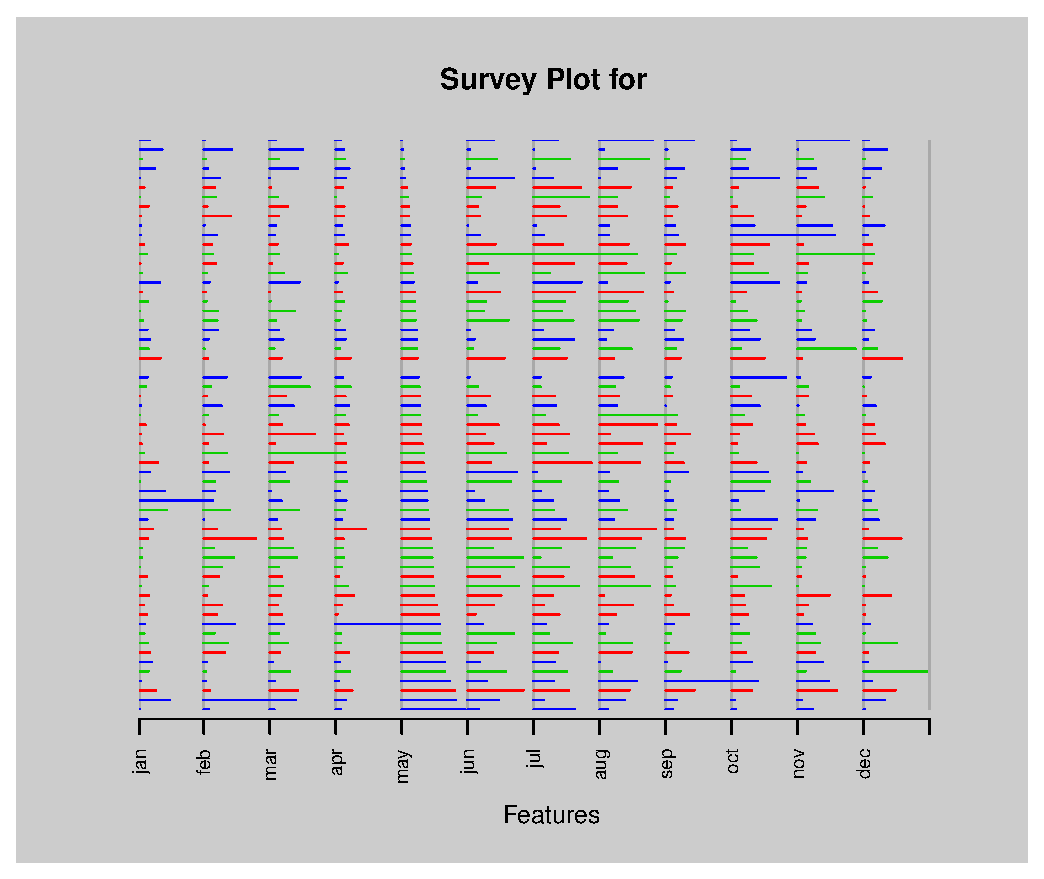
\includegraphics[width = \textwidth]{3cii5.eps}
        	\caption{May}
        	\end{subfigure}%
        	\begin{subfigure}[b]{0.3\textwidth}
        	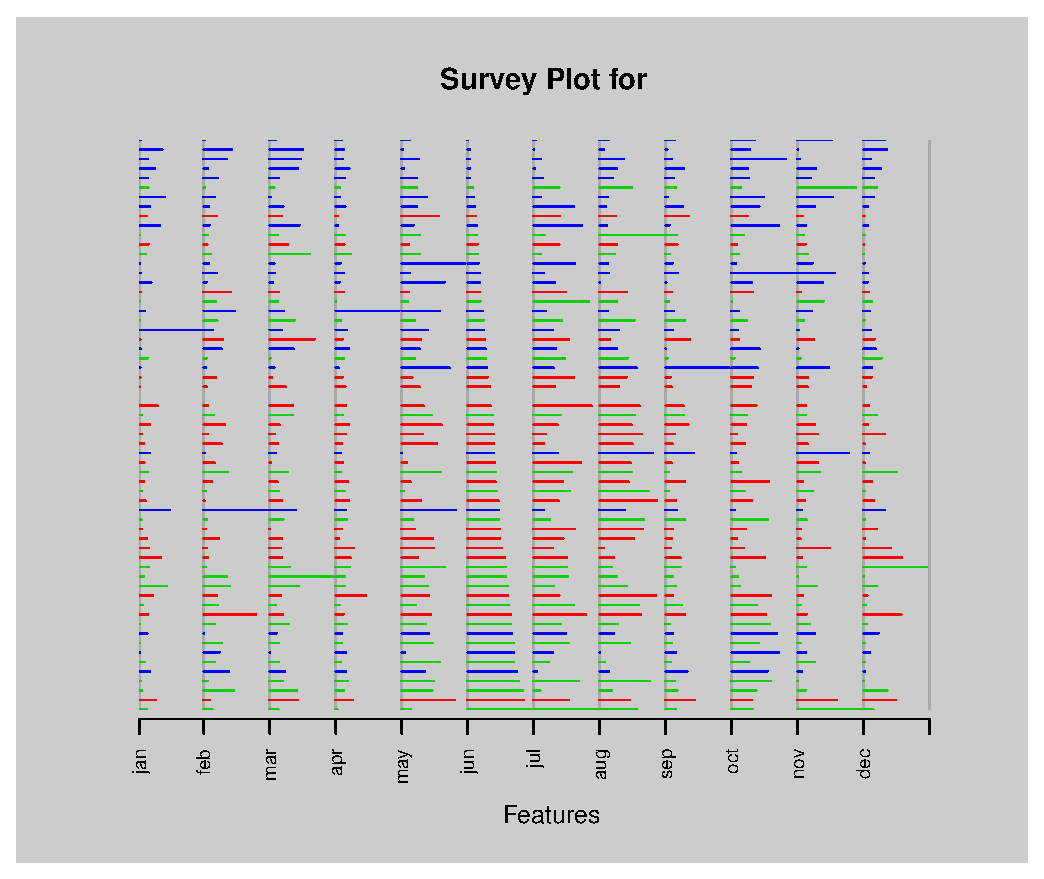
\includegraphics[width = \textwidth]{3cii6.eps}
        	\caption{Jun}
        	\end{subfigure}\\           
        	\begin{subfigure}[b]{0.3\textwidth}
        	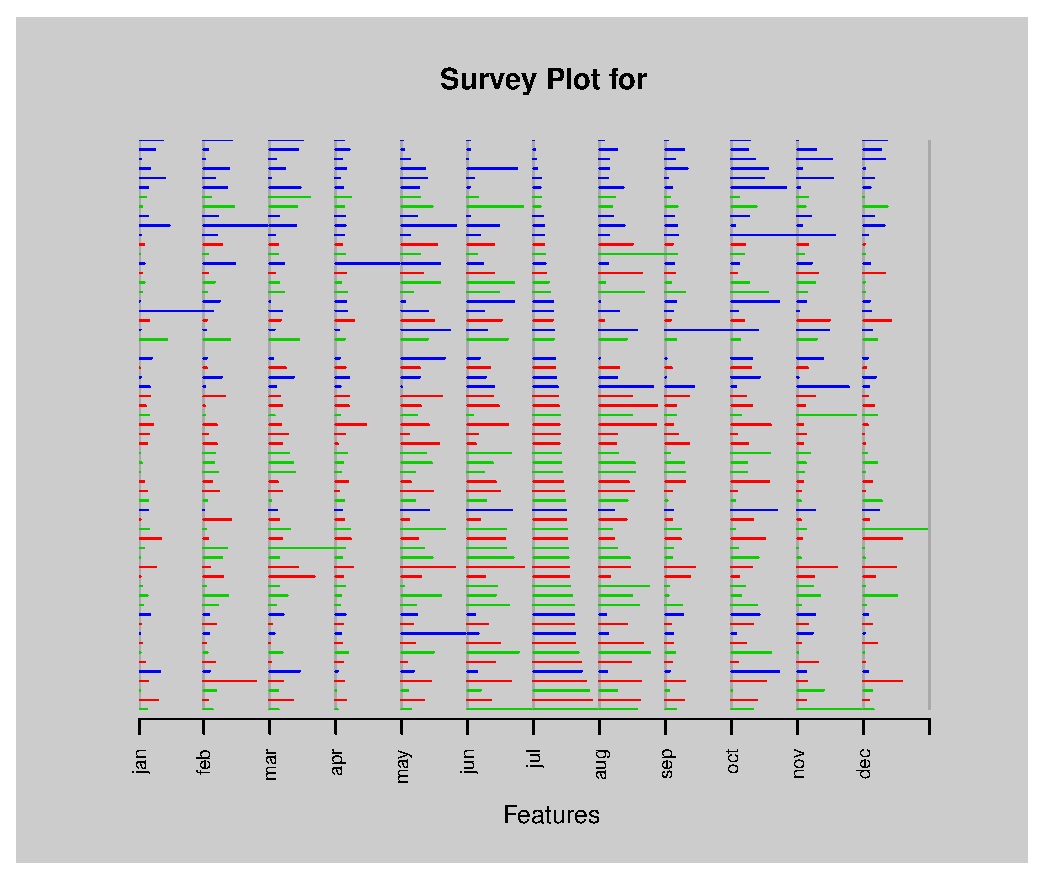
\includegraphics[width = \textwidth]{3cii7.eps}
        	\caption{Jul}
        	\end{subfigure}%
        	\begin{subfigure}[b]{0.3\textwidth}
        	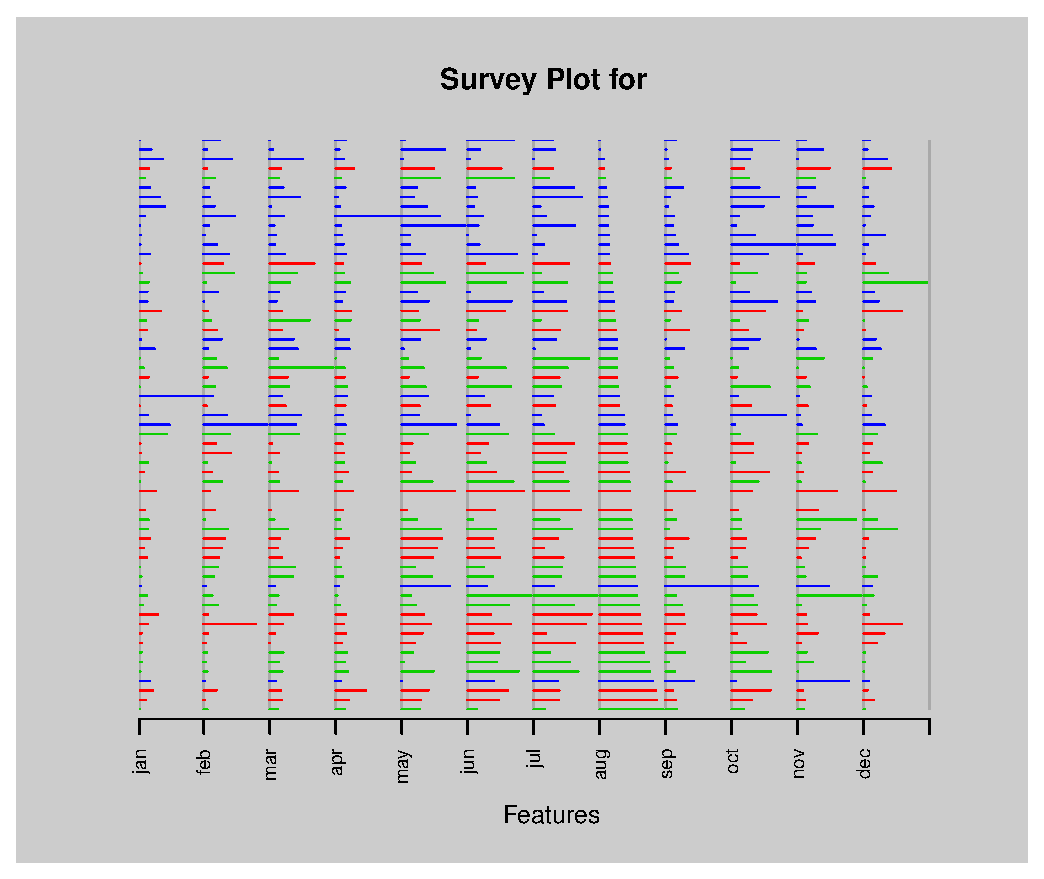
\includegraphics[width = \textwidth]{3cii8.eps}
        	\caption{Aug}
        	\end{subfigure}%
        	\begin{subfigure}[b]{0.3\textwidth}
        	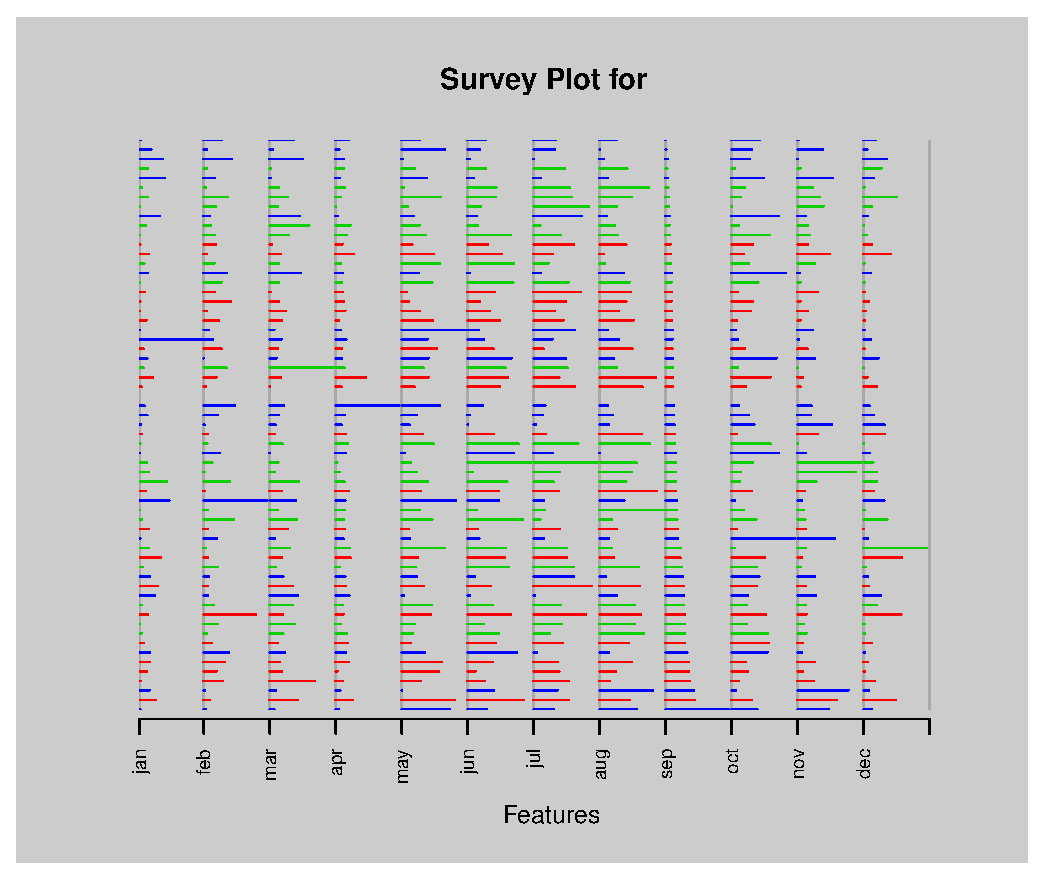
\includegraphics[width = \textwidth]{3cii9.eps}
        	\caption{Sept}
        	\end{subfigure}\\
        	\begin{subfigure}[b]{0.3\textwidth}
        	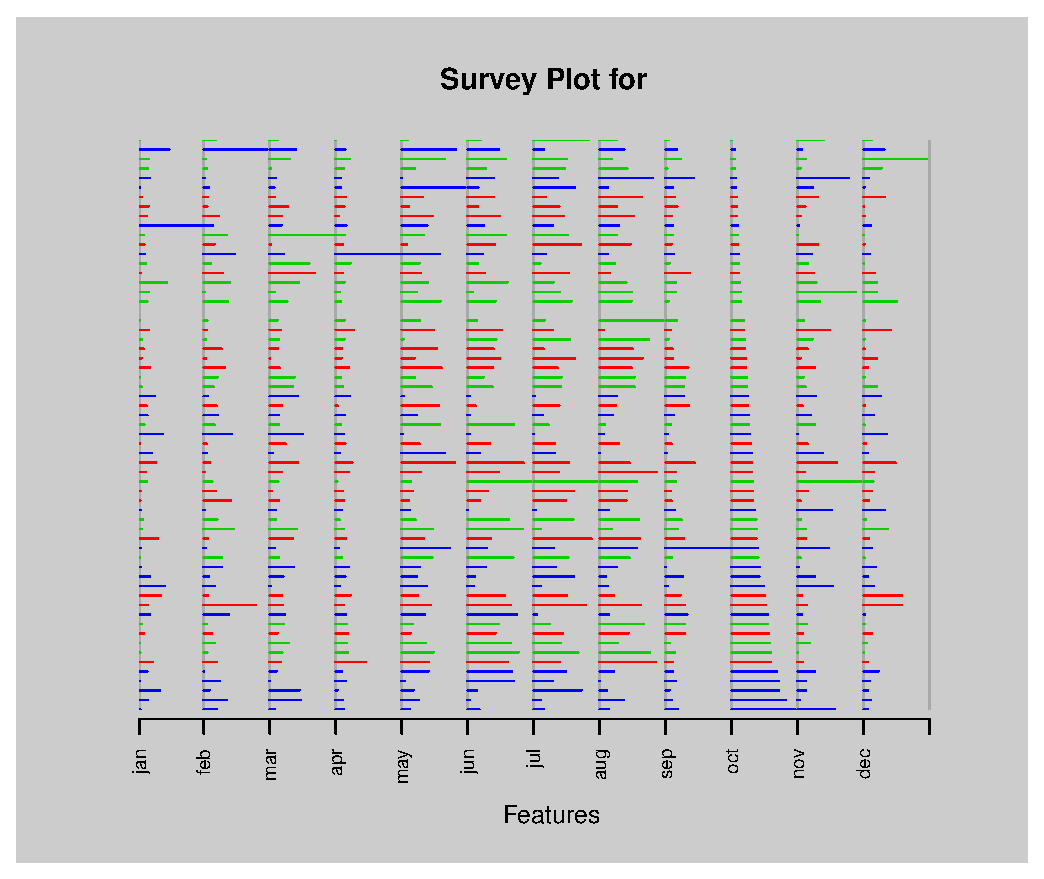
\includegraphics[width = \textwidth]{3cii10.eps}
        	\caption{Oct}
        	\end{subfigure}%
        	\begin{subfigure}[b]{0.3\textwidth}
        	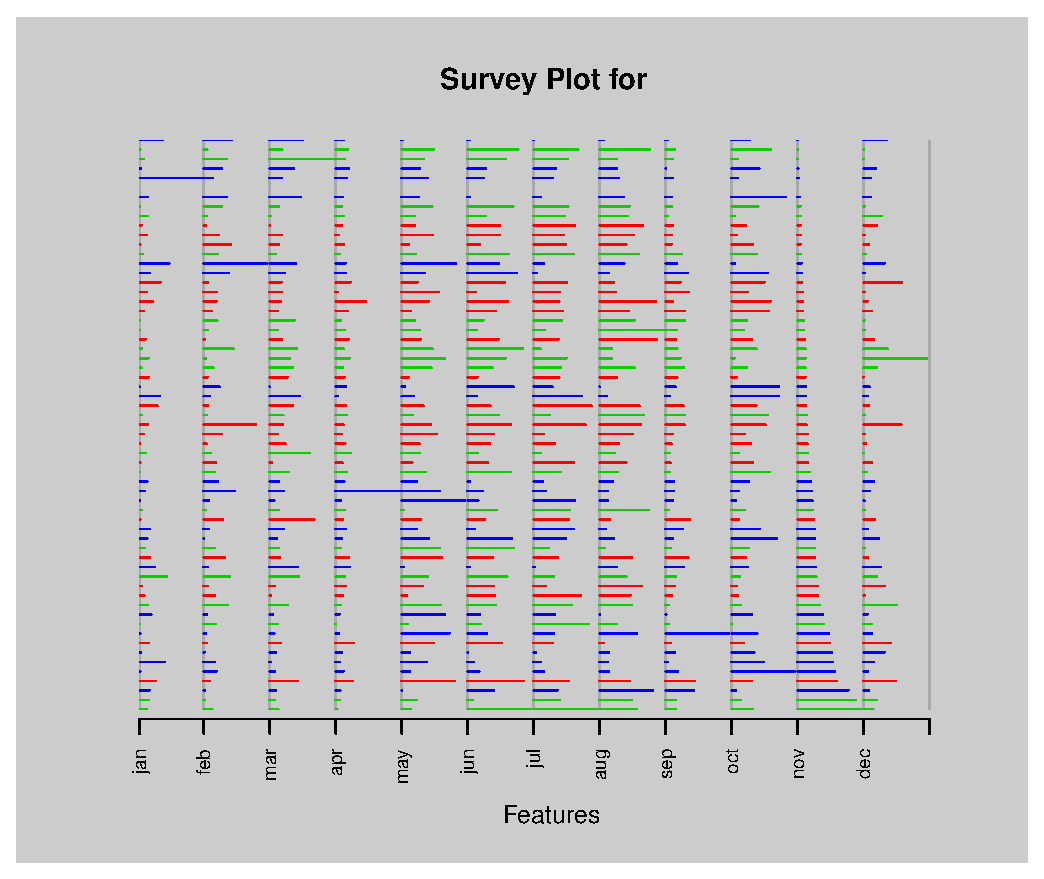
\includegraphics[width = \textwidth]{3cii11.eps}
        	\caption{Nov}
        	\end{subfigure}%
        	\begin{subfigure}[b]{0.3\textwidth}
        	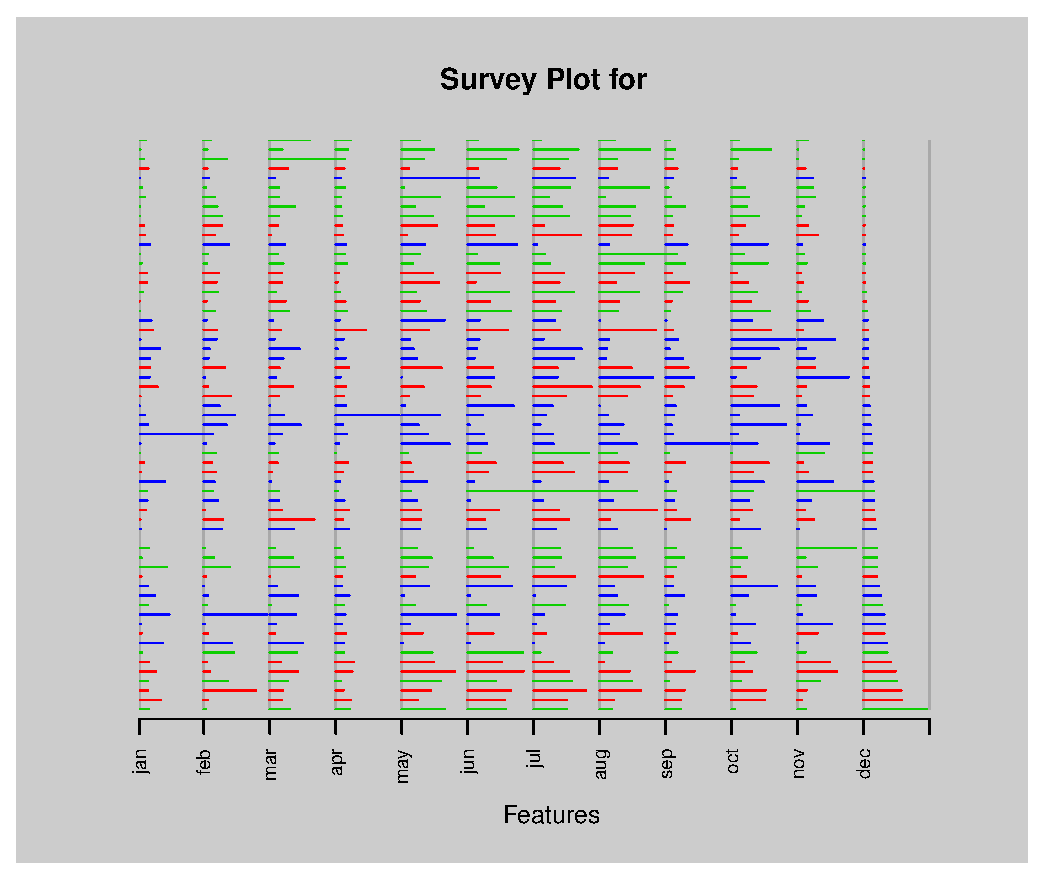
\includegraphics[width = \textwidth]{3cii12.eps}
        	\caption{Dec}
        	\end{subfigure}
        	\caption{survey plots with different orders}
        	\label{3bii}
        \end{figure}
        \newpage
        The survey plots with 12 different orders are shown in Figure~\ref{3bii}. From the survey plot distinct patterns were not visible and ordering by none of the month provided a clear separation between the classes
        \newpage
        \item 
        Create the stars and Chernoff faces plot for the mean of three group
        \begin{rcode}
library(TeachingDemos)
# Compute the mean for three groups
Means<-aggregate(x = Tornado[-1,2:13],by=list(Tornado$Period[-1]),FUN = mean)

#Create chernoff face for the means
faces(xy = Means[,2:13])
#Create stars for the group means
stars(x = Means[,2:13],labels = as.character(Means$Group.1),scale = T,full = T,radius = T) 	
        \end{rcode}
        Plot of Chernoff faces is shown in Figure~\ref{3biiifaces} and stars in shown in Figure~\ref{3biiistars}. From both Chernoff face and stars, differences are observed between the group means.
        \begin{figure}[!htb]
        	\centering
        	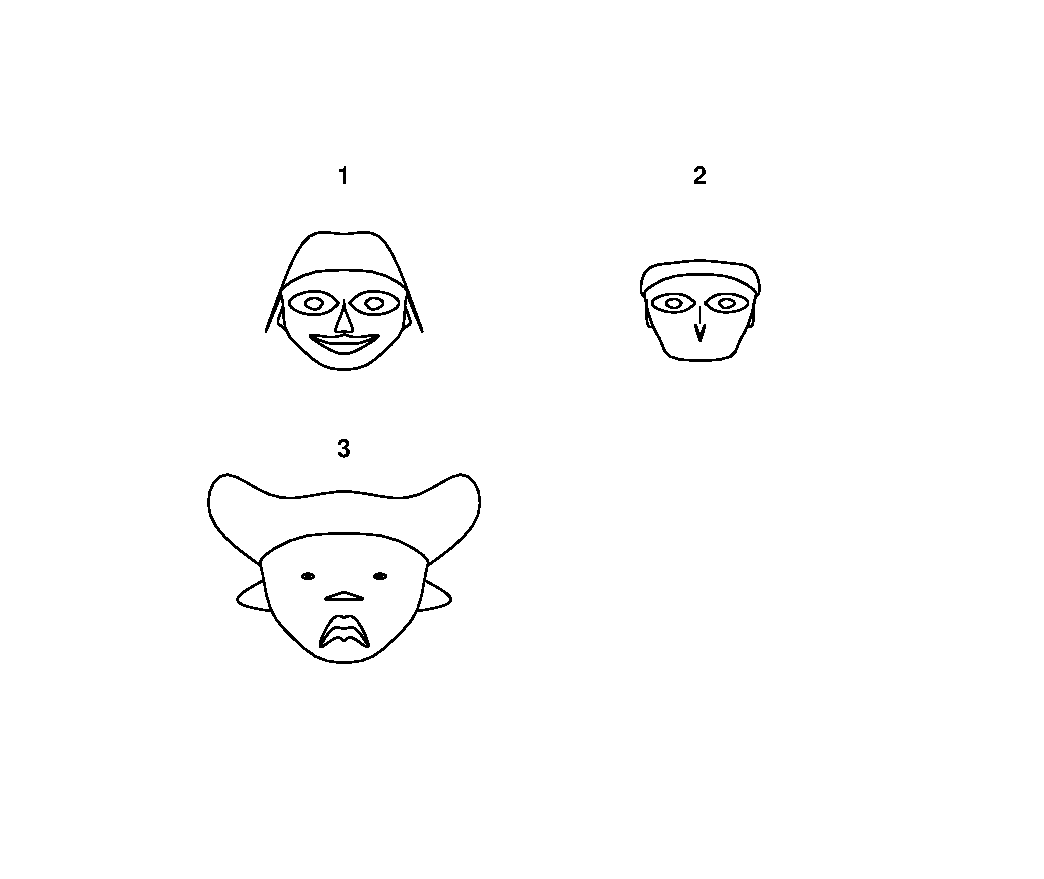
\includegraphics[width = 0.5\textwidth]{3ciiiface.eps}
        	\caption{Chernoff faces for Tornado data}
        	\label{3biiifaces}
        \end{figure}

        \begin{figure}[!htb]
        	\centering
        	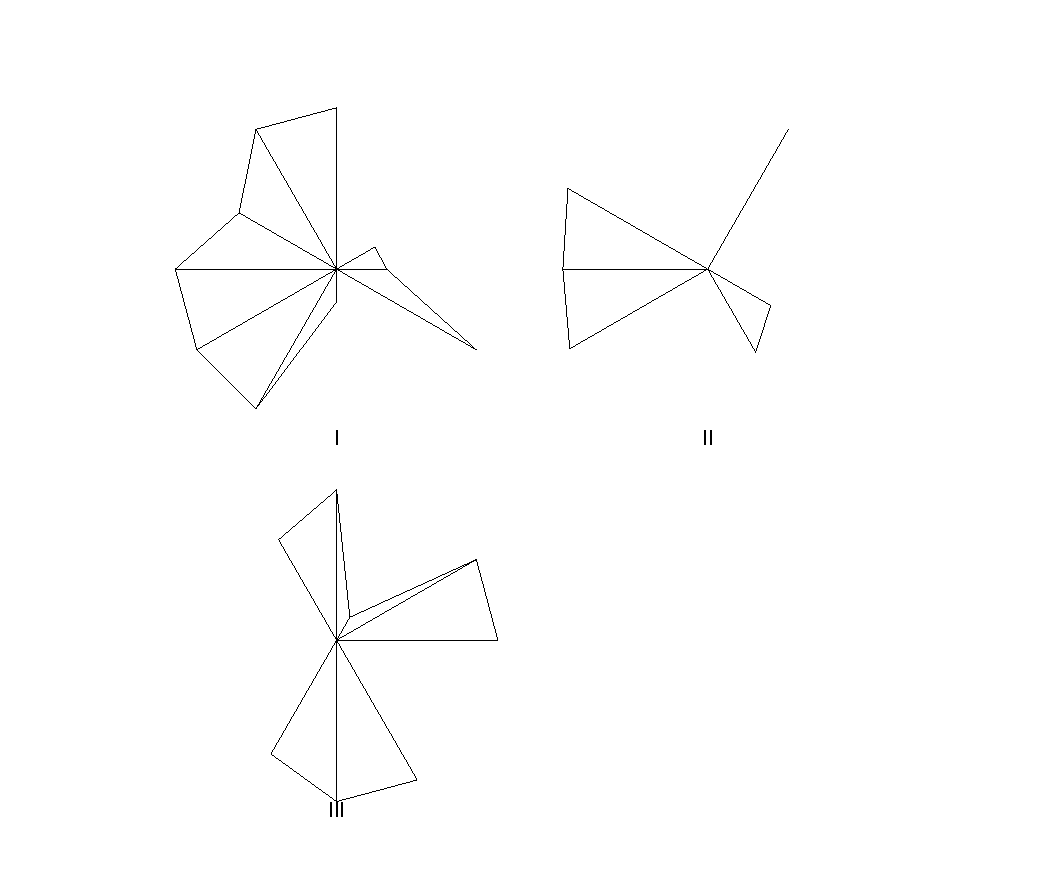
\includegraphics[width = 0.5\textwidth]{3ciiistars.eps}
        	\caption{Stars for Tornado data}
        	\label{3biiistars}
        \end{figure}
		\end{enumerate}

		
	\end{enumerate}
	\newpage
	\item 
	Let $\bm a = \bm X - \bm X^T \bm 1/p,\bm b =  \bm Y - \bm Y^T \bm 1 /p$. Then 
	\[\|\bm X^{\circ} - \bm Y^{\circ}\|^2 = \left\|\frac{\bm a}{\|\bm a\|} - \frac{\bm b}{\|\bm b\|}\right\|^2 = \inner{\frac{\bm a}{\|\bm a\|} - \frac{\bm b}{\|\bm b\|}}{\frac{\bm a}{\|\bm a\|} - \frac{\bm b}{\|\bm b\|}},\]
	where $\inner{\cdot}{\cdot}$ is inner product.

	Since $\mathrm{Var}(\bm X) = \sum_{i = 1}^p (x_i - \bar{x})^2 = \|\bm X - \bm X^T \bm 1/p\|^2 = \|\bm a\|^2, \, \mathrm{Var}(\bm Y) = \sum_{i = 1}^p (y_i - \bar{y})^2 = \|\bm Y - \bm Y^T \bm 1/p\|^2 = \|\bm b\|^2$ and $\mathrm{Cov}(\bm X, \bm Y) = \sum_{i=1}^p (x_i - \bar{x})(y_i - \bar{y}) = \inner{\bm X - \bm X^T\bm 1/p}{\bm Y - \bm Y^T\bm 1/p} = \inner{\bm a}{\bm b}.$ Hence
	\[\mathrm{Corr}(\bm X, \bm Y) = \frac{\mathrm{Cov}(\bm X, \bm Y)}{\sqrt{\mathrm{Var}(\bm X)}\sqrt{\mathrm{Var}{\bm Y}}} = \frac{\inner{\bm a}{\bm b}}{\|\bm a\|\|\bm b\|}\]

	Thus 
	\begin{align*}
	\|\bm X^{\circ} - \bm Y^{\circ}\|^2 &= \inner{\frac{\bm a}{\|\bm a\|} - \frac{\bm b}{\|\bm b\|}}{\frac{\bm a}{\|\bm a\|} - \frac{\bm b}{\|\bm b\|}}\\
	& = \inner{\frac{\bm a}{\|\bm a\|}}{\frac{\bm a}{\|\bm a\|}} + \inner{\frac{\bm b}{\|\bm b\|}}{\frac{\bm b}{\|\bm b\|}} - 2 \inner{\frac{\bm a}{\|\bm a\|}}{\frac{\bm b}{\|\bm b\|}}\\
	& = \frac{\|\bm a\|^2}{\|\bm a\|^2} + \frac{\|\bm b\|^2}{\|\bm b\|^2} - \frac{2 \inner{\bm a}{\bm b}}{\|\bm a\|\|\bm b\|}\\
	& = 2 - 2 \mathrm{Corr}(\bm X, \bm Y)
	\end{align*}


 	\end{enumerate}






	
	
	
	\end{document}